% Copyright 2004 by Till Tantau <tantau@users.sourceforge.net>.
%
% In principle, this file can be redistributed and/or modified under
% the terms of the GNU Public License, version 2.
%
% However, this file is supposed to be a template to be modified
% for your own needs. For this reason, if you use this file as a
% template and not specifically distribute it as part of a another
% package/program, I grant the extra permission to freely copy and
% modify this file as you see fit and even to delete this copyright
% notice. 

\documentclass{beamer}
\usepackage{graphicx}
\usepackage{breqn}
\graphicspath{ {images/Eric/} }
\usepackage{amsmath}
\usepackage{dsfont}
% There are many different themes available for Beamer. A comprehensive
% list with examples is given here:
% http://deic.uab.es/~iblanes/beamer_gallery/index_by_theme.html
% You can uncomment the themes below if you would like to use a different
% one:
%\usetheme{AnnArbor}
%\usetheme{Antibes}
%\usetheme{Bergen}
%\usetheme{Berkeley}
\usetheme{Berlin}
%\usetheme{Boadilla}
%\usetheme{boxes}
%\usetheme{CambridgeUS}
%\usetheme{Copenhagen}
%\usetheme{Darmstadt}
%\usetheme{default}
%\usetheme{Frankfurt}
%\usetheme{Goettingen}
%\usetheme{Hannover}
%\usetheme{Ilmenau}
%\usetheme{JuanLesPins}
%\usetheme{Luebeck}
%\usetheme{Madrid}
%\usetheme{Malmoe}
%\usetheme{Marburg}
%\usetheme{Montpellier}
%\usetheme{PaloAlto}
%\usetheme{Pittsburgh}
%\usetheme{Rochester}
%\usetheme{Singapore}
%\usetheme{Szeged}
%\usetheme{Warsaw}

\title{Effects of Unemployment Benefits and Uncertainty in Heterogeneous Models}

% A subtitle is optional and this may be deleted
\subtitle{}

\author{Eric, Yannic and Andrian}
% - Give the names in the same order as the appear in the paper.
% - Use the \inst{?} command only if the authors have different
%   affiliation.

%\institute[Universities of Somewhere and Elsewhere] % (optional, but mostly needed)
%{
% \inst{1}%
%  Department of Computer Science\\
%  University of Somewhere
%  \and
%  \inst{2}%
%  Department of Theoretical Philosophy\\
%  University of Elsewhere}
% - Use the \inst command only if there are several affiliations.
% - Keep it simple, no one is interested in your street address.

%\date{Conference Name, 2013}
% - Either use conference name or its abbreviation.
% - Not really informative to the audience, more for people (including
%   yourself) who are reading the slides online

%\subject{Theoretical Computer Science}
% This is only inserted into the PDF information catalog. Can be left
% out. 

% If you have a file called "university-logo-filename.xxx", where xxx
% is a graphic format that can be processed by latex or pdflatex,
% resp., then you can add a logo as follows:

% \pgfdeclareimage[height=0.5cm]{university-logo}{university-logo-filename}
% \logo{\pgfuseimage{university-logo}}

% Delete this, if you do not want the table of contents to pop up at
% the beginning of each subsection:
\AtBeginSubsection[]
{
  \begin{frame}<beamer>{Outline}
    \tableofcontents[currentsection,currentsubsection]
  \end{frame}
}


% Let's get started
\begin{document}



\begin{frame}
  \titlepage
\end{frame}

\begin{frame}{Outline}
  \tableofcontents
  % You might wish to add the option [pausesections]
\end{frame}

% Section and subsections will appear in the presentation overview
% and table of contents.
\section{Changes in idiosyncratic risk}

\begin{frame}{Questions}
	\begin{itemize}
	
	\item {
	Does idiosyncratic risk matter? How do changes in such risk affect other economic variables? Are there distributional consequences?
	}
	
	\end{itemize}
\end{frame}

\begin{frame}{How do we examine these questions?}
	\begin{itemize}
	
	\item {
	We will look at changes in the unemployment benefit. 
	}
		
	\end{itemize}
\end{frame}

\subsection{The model}
\begin{frame}{Model Summary}
	\begin{itemize}
	
	\item {
	Ex ante identical individuals are subject to uninsurable idiosyncratic shocks. 
	}
	\item {
Agents can interact on the asset market.
	}
	\item {
The model generates an endogenous distribution of wealth across consumers. 
	}	
	\item {
Aggregates and prices are jointly determined by the saving behavior of the collection of all households. 
}

	\end{itemize}

\end{frame}


\subsection{Changes in the unemployment insurance}

\begin{frame}{Different parameters of the model}


  \centering{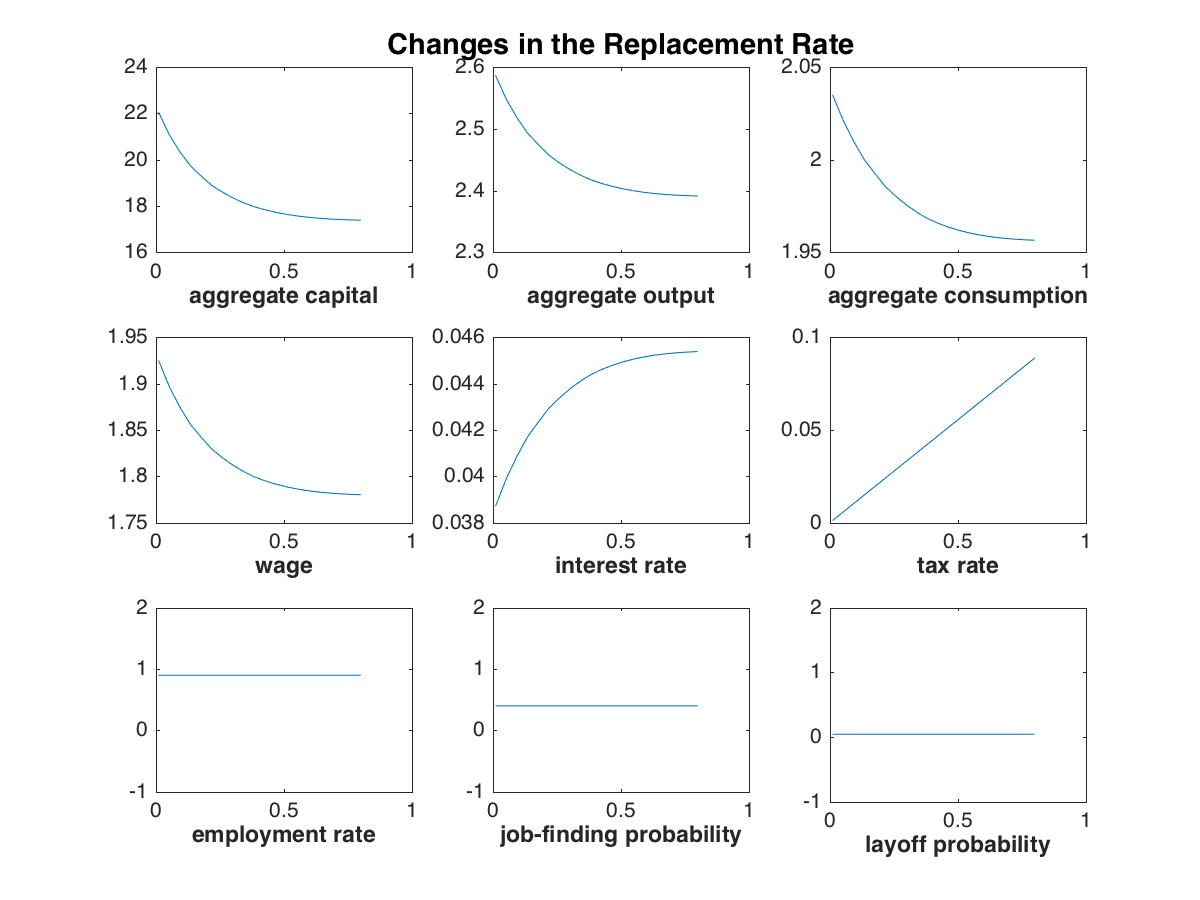
\includegraphics[scale=0.45]{parameters}}


\end{frame}

\begin{frame}{Different levels of risk aversion}


  \centering{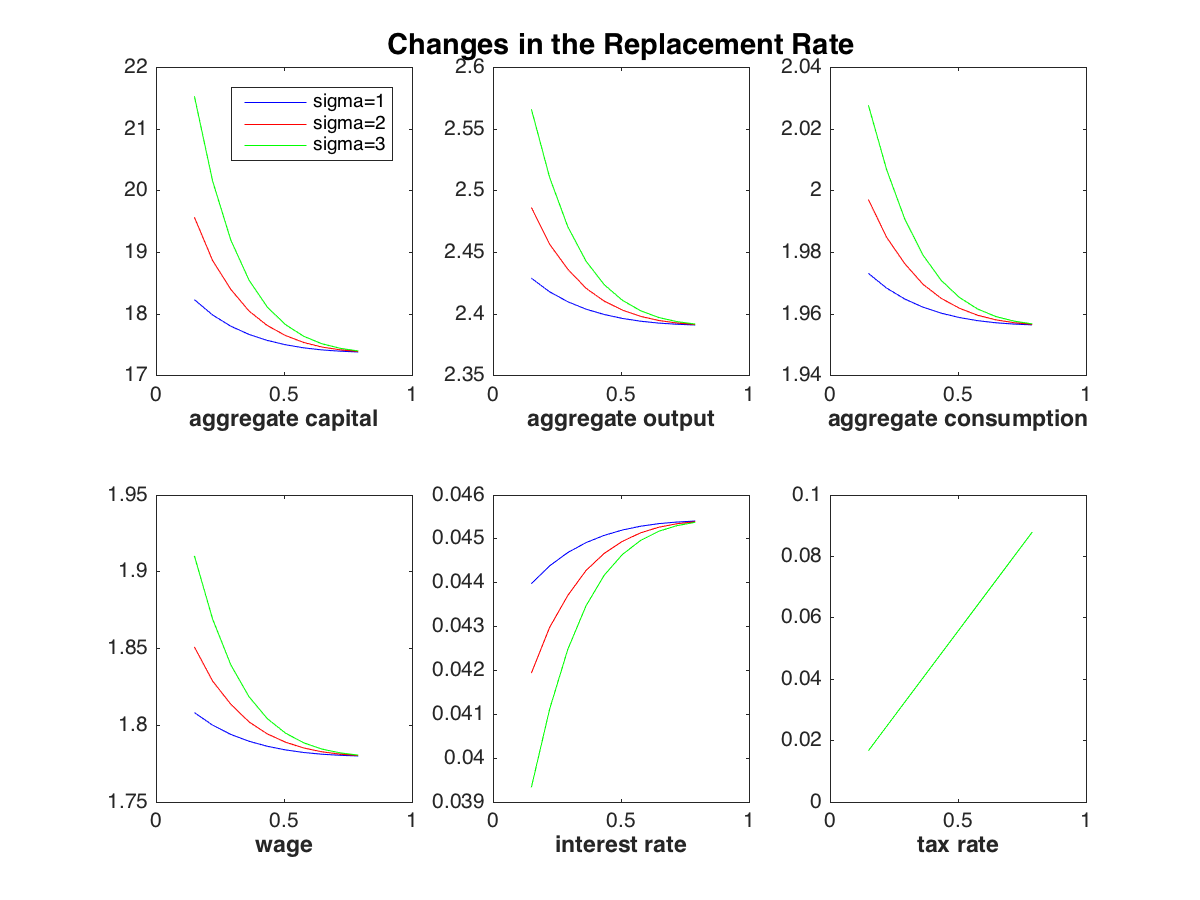
\includegraphics[scale=0.45]{parameters_sigma}}


\end{frame}


\begin{frame}{First Observations}
	\begin{itemize}
	
	\item {
	Changes in idiosyncratic risk do affect aggregate variables.
	}

	\item {
	The magnitude of impact varies for different levels of risk aversion.
	}
	
		\item {
	How do the different levels of the aggregates compare to a situation with perfect insurance? 
	}

	\end{itemize}
	
\end{frame}
	

\begin{frame}{Comparing to complete markets}
  \centering{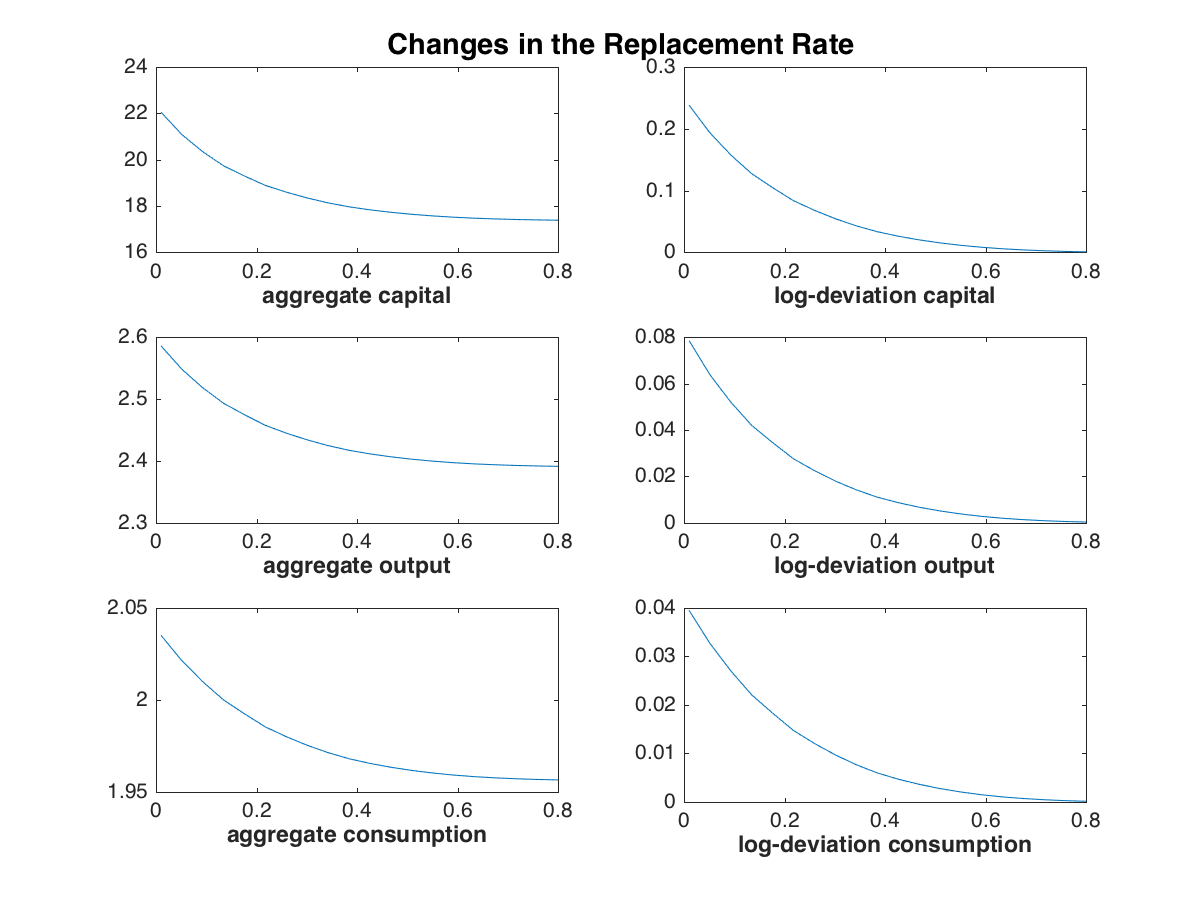
\includegraphics[scale=0.45]{log-deviation}}

\end{frame}
	
		
\begin{frame}{Comparing to complete markets}
	\begin{itemize}
	
	\item {
	As the insurance increases, the aggregates converge to the levels of the complete market economy. 
	}


	\end{itemize} 
\end{frame}



\begin{frame}{Distribution of capital}
 
\begin{figure}[!tbp]
  \centering
  \begin{minipage}[b]{0.325\textwidth}
    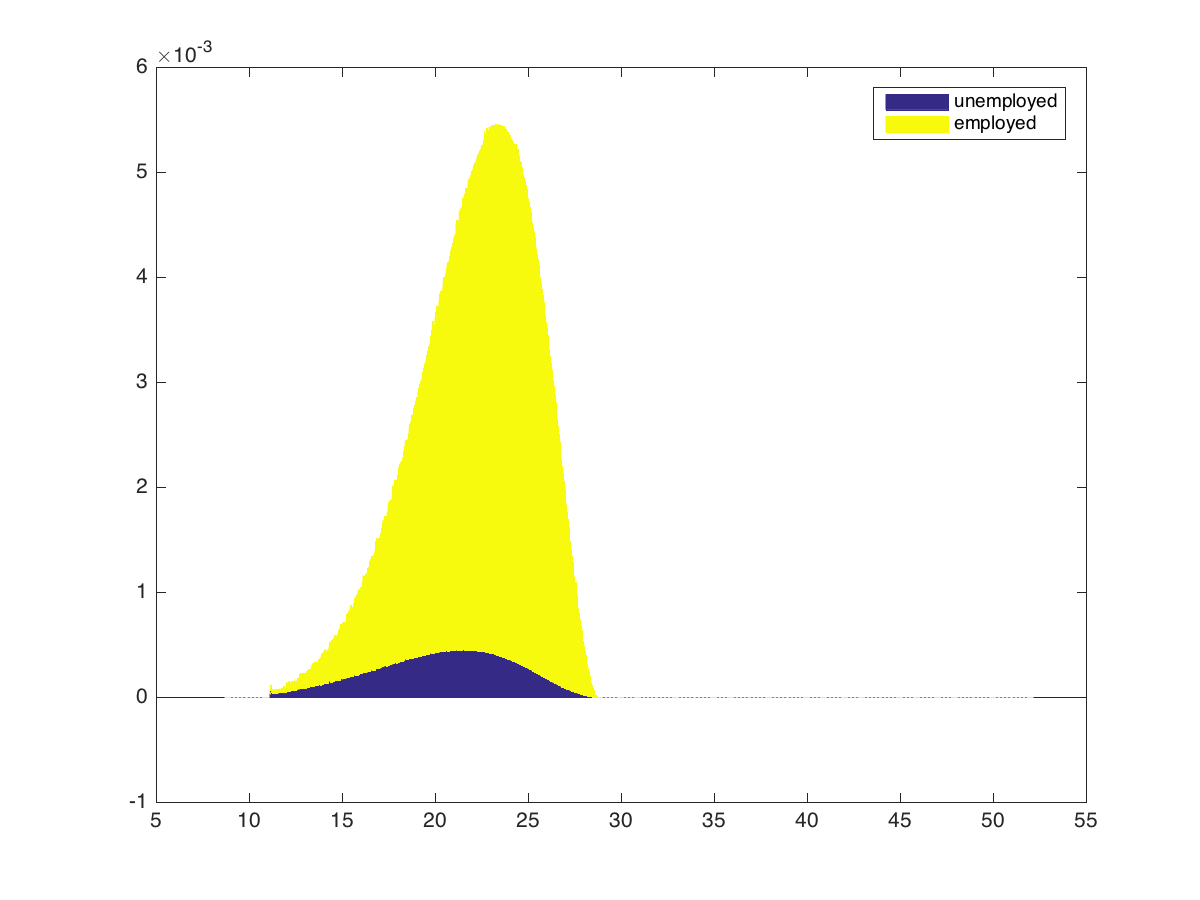
\includegraphics[width=\textwidth]{distribution1}
  \end{minipage}
  \hfill
  \begin{minipage}[b]{0.325\textwidth}
    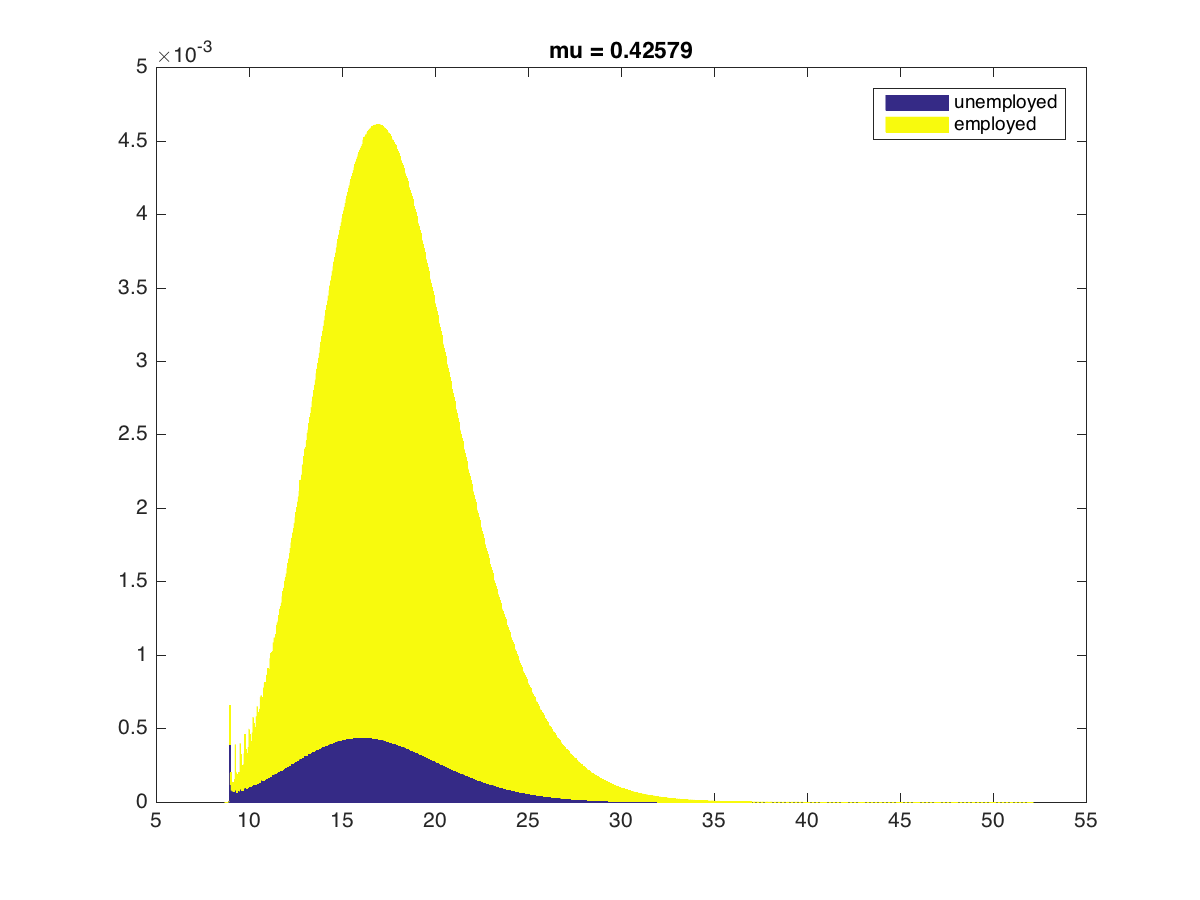
\includegraphics[width=\textwidth]{distribution2}
  \end{minipage}
  \hfill
  \begin{minipage}[b]{0.325\textwidth}
    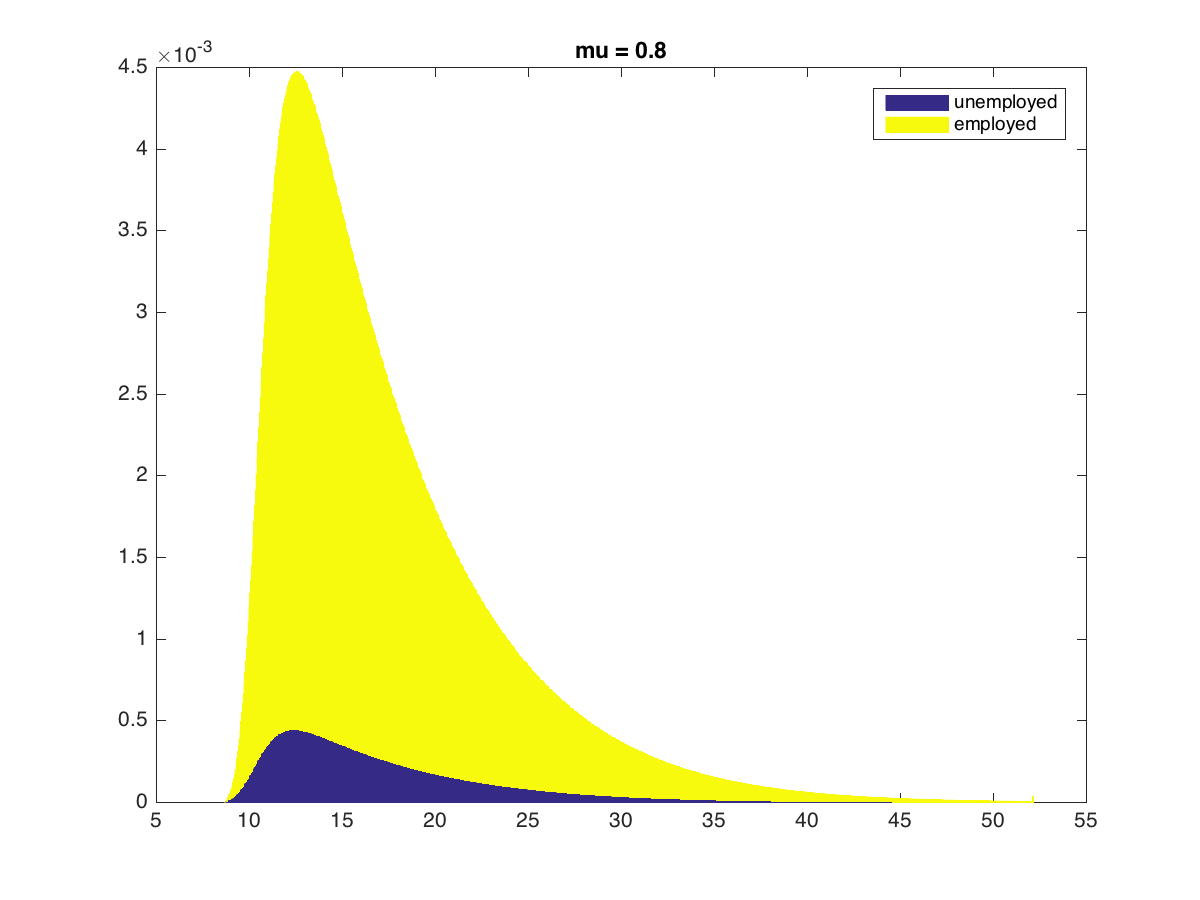
\includegraphics[width=\textwidth]{distribution3}
  \end{minipage}
\end{figure}
\ \ \ \ \ \ \  rw = 0.01 \ \ \ \ \ \ \ \ \ \ \ \ rw = 0.42579 \ \ \ \ \ \ \ \ \ \ \ \ \ rw = 0.8
\end{frame}


\begin{frame}{Concluding on the distribution}

\begin{itemize} 


	\item {
As precautionary savings decrease, aggregate capital decreases, thus increasing the interest rate and reducing the wage. 
}
	\item {
The increase in unemployment benefits further reduces the net wage of the employed. The government has to increase income taxes to finance the higher unemployment benefits.
}
	\item {
Therefore, with higher unemployment benefits the agent's income depends more on his accumulated capital than his labor or benefits income. 
}
	\item {
The dispersion of the distribution therefore increases as benefits increase.
}


\end{itemize}

\end{frame}


\begin{frame}{Concluding the first part}
	
	\begin{itemize}
	
	\item {
Idiosyncratic risk matters: 
Precautionary savings increase with higher uncertainty, thus increasing aggregate capital. 
	}	
	\item {
Increasing unemployment benefits has distributional consequences. 
	}	

	\end{itemize} 
\end{frame}

\begin{frame}{The limitations}
	
	\begin{itemize}
	
	\item {The model's labor supply is exogenous. Thus, changing the unemployment benefits has no impact on labor supply or the transition probabilities.
}	
	\item {This contradicts empirical evidence: Decker(1997).
	}
	\item{Endogenous labor matters: Mukoyama(2012).
	}

	\end{itemize} 
\end{frame}


\section{Welfare effects}
\subsection{}


\section{Aggregate risk}
\subsection{}

\section{Conclusions}
\subsection{}

\end{document}